% ------------------------------------------------------------------------------
% In the design section a general overview about the system to be implemented is
% shown. All the hardware, software, communications and other topics are
% evaluated and selected.
% ------------------------------------------------------------------------------

\opt{never}{\addbibresource{03-tail/bibliography.bib}} % to make citation found in most IDE

\chapter{Design}
\label{chap:design}

% -- Your text goes here --
The design phase provides an overview of the various components of the reference architecture. It sets out the conceptualisation of the structure of the \gls{cloud_infrastructure} with the integration of multiple embedded systems. An overview of the automation process is presented, as well as an explanation of the general operation of each application included in this architecture.

\minitoc
\newpage

% ------------------------------------------------------------------------------
\section{Reference architecture}

% -- Your text goes here --
The reference architecture is divided into two parts: the first concerns embedded systems based on \gls{arm} architectures and certified \nameref{sec:arm_systemready} with a Linux \acrlong{os}, while the second relates to the \gls{cloud} and is hosted by the \gls{aws} provider. An overview is clearly shown in figure \ref{fig:RefArch_Overview}.
\begin{center}
    \begingroup
    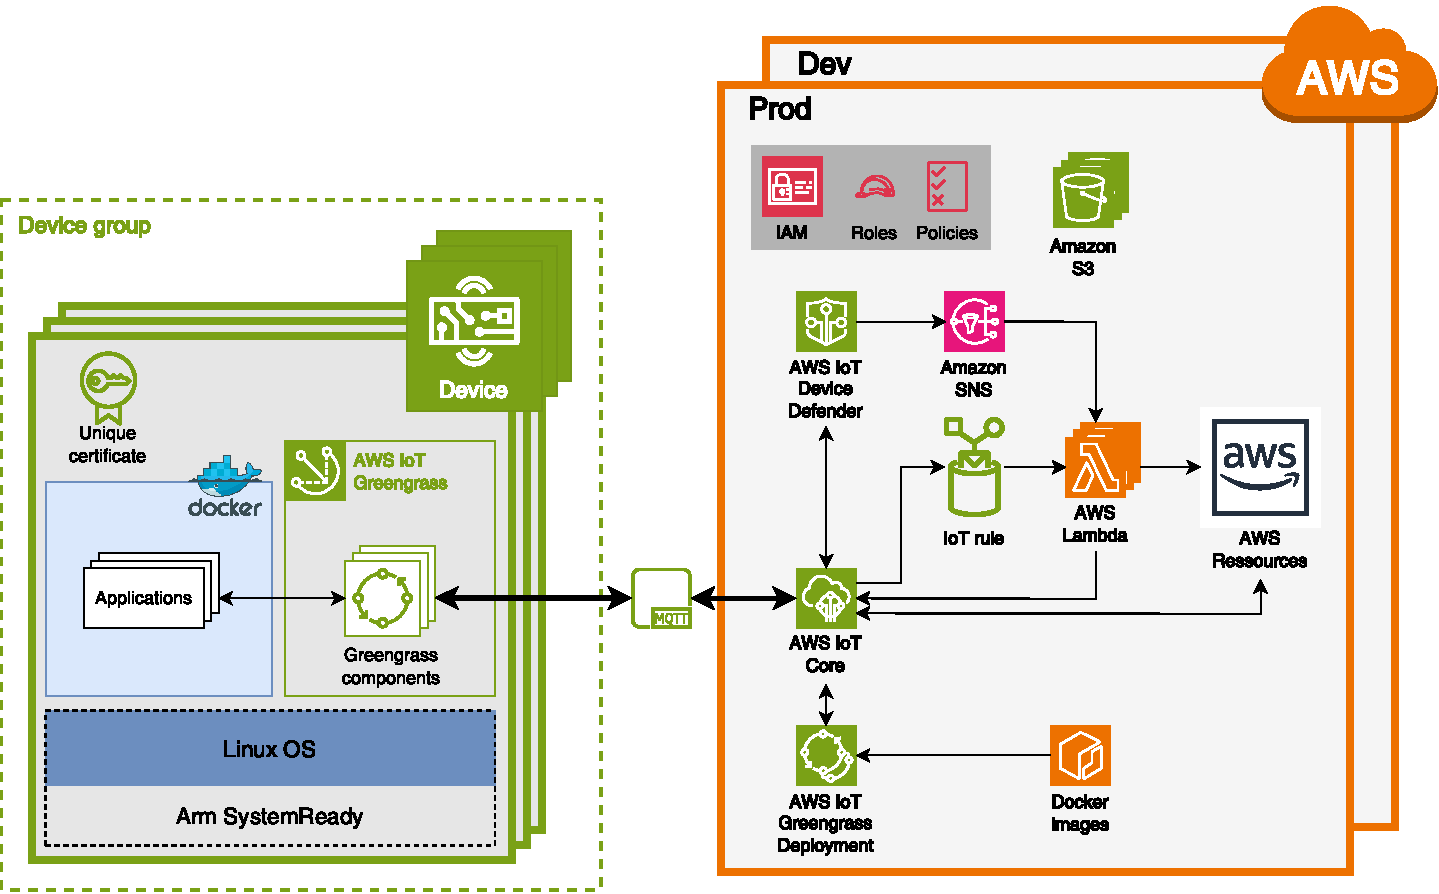
\includegraphics[width=1\columnwidth]{design/RefArch_Overview.pdf}
    \captionof{figure}{Reference architecture overview}
    \label{fig:RefArch_Overview}
    \endgroup
\end{center}

\subsection{\Gls{cloud_infrastructure}}
In the \gls{cloud}, two distinct infrastructures are presented. The first infrastructure is dedicated to development, enabling all kinds of operations to be tested. The second infrastructure is the production infrastructure, encompassing the final product intended for customers. Each infrastructure uses different \gls{aws} services.

The central service managing the \acrshort{iot} is \gls{aws} \acrshort{iot} Core, which exchanges data with all connected devices. Its preferred communication protocol is \acrshort{mqtt}. Provisioned devices are registered in a specific group within this service. Only authorised devices are provisioned. \gls{aws} \acrshort{iot} Greengrass Deployment handles the deployment of new Greengrass components or updates to a group of devices. A component, in the context of \gls{aws} \acrshort{iot} Greengrass, is a unit of deployment and execution that encapsulates code, dependencies and resources, making it easy to deploy, manage and update \acrshort{iot} applications. In this architecture, Docker components are used, encapsulating containers to offer greater flexibility in software deployment. Docker images are stored in the Amazon \acrfull{ecr}. Another service, \gls{aws} \acrshort{iot} Device Defender, checks daily whether a certificate is about to expire, as each device has a unique certificate enabling a secure connection. If a certificate expires within 30 days, it is replaced by a new one. Other Lambda functions, triggered by rules, can enrich the architecture, as can other \gls{aws} resources, depending on the needs of each developer. Storage spaces such as Amazon S3 are used to save the state of the infrastructure, configuration files for device \gls{provisioning} and \acrshort{os} images. The configuration files contain a list of the serial numbers of all the \acrshort{iot} devices authorised to be provisioned. If a device is not listed and attempts to be provisioned, access will be denied. If a device is already provisioned and its serial number is removed from the list, its access will be withdrawn and it will be deleted from the \gls{cloud}. The IAM service is there to assign roles and policies, limiting authorised actions on resources to the strict minimum.

\subsection{Embedded systems integration}
Embedded systems must be based on \gls{arm} architecture and be \nameref{sec:arm_systemready} certified. The devices are flashed with a custom Linux \acrshort{os} image. On first boot, two software programs are installed : Docker Engine for running Docker containers, and \gls{aws} \acrshort{iot} Greengrass Core for \gls{provisioning}, communicating with \gls{aws} \acrshort{iot} Core and managing Greengrass components. This software provisions the device by exchanging the claim certificate with a unique certificate, securing the connection of the device, which is then registered in the device group. Deployment of Greengrass components from the \gls{cloud} to devices is automated when a new device is associated or a new version of a component becomes available. Applications are contained in Docker containers to ensure optimum portability.


% ------------------------------------------------------------------------------
\section{\texorpdfstring{\acrshort{ci}/\acrshort{cd}}{} pipeline}

% -- Your text goes here --
The pipeline is made up of several workflows, each dedicated to a specific function. An overview of the various stages in the pipeline is shown in figure \ref{fig:CICD_Pipeline_Overview}. The pipeline uses \acrshort{ci}/\acrshort{cd} methods to automate the deployment of the \gls{cloud_infrastructure}, as well as preparing for the integration of embedded systems.
\begin{center}
    \begingroup
    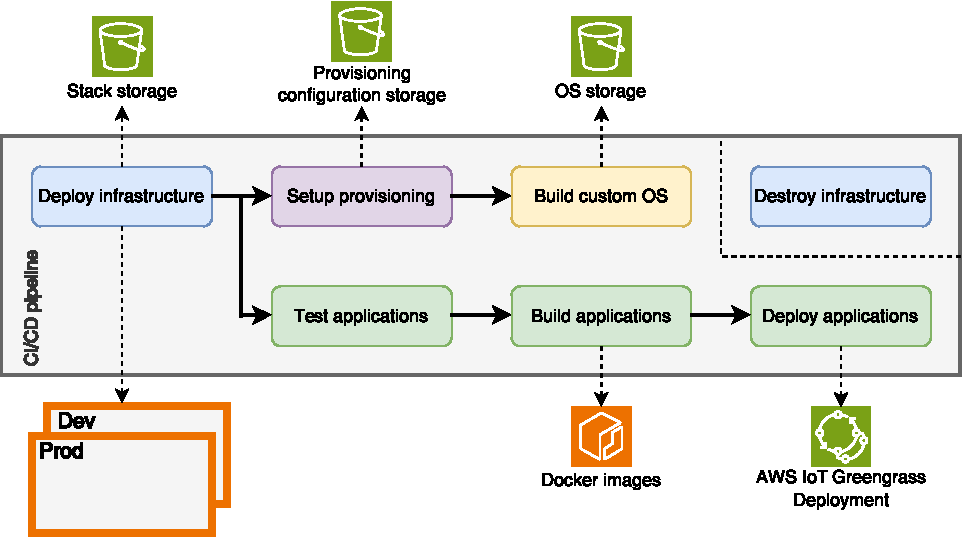
\includegraphics[width=1\columnwidth]{design/CICD_Pipeline_Overview.pdf}
    \captionof{figure}{\acrshort{ci}/\acrshort{cd} workflows overview}
    \label{fig:CICD_Pipeline_Overview}
    \endgroup
\end{center}
The first job is to deploy the \gls{aws} \gls{cloud_infrastructure} (\textit{Deploy infrastructure}). It can enable the deployment of development or production infrastructure. Since it uses a tool called \acrshort{iac}, the state of the infrastructure must be stored. This flow also enables resources to be updated.

If the entire infrastructure is deployed without error, the \gls{provisioning} configuration workflow (\textit{Setup \gls{provisioning}}) takes care of preparing configuration files for \gls{provisioning} in a storage space. It also manages device control. It checks the list of authorised devices to identify whether a previously provisioned device has been removed from the list. If so, it will be removed from the \gls{cloud}. It may also be the case that authorised devices have already been provisioned and need to be connected to the new infrastructure. This operation is also checked and carried out.

If the previous step has been successful, the next step (\textit{Build custom \acrshort{os}}) is to prepare and create the \acrshort{os} image with all the files and scripts needed to automatically provision the devices when they start up for the first time. The image must be saved in a storage space that allows it to be downloaded for flashing the devices' SD cards.

In parallel with the previous two workflows, the application workflows are launched. The first (\textit{Test applications}) performs various tests on the applications. It includes security and unit tests.

If the tests have not failed, the next job (\textit{Build applications}) is to build the Greengrass components from the applications. A Docker image is first created for each of the applications, coded in a freely chosen programming language. These images are then linked to their respective components. Finally, the components must be saved in the \gls{aws} \acrshort{iot} Greengrass service to be ready for deployment.

The last flow (\textit{Deploy applications}) takes care of deploying applications to the device group. It uses the \gls{aws} \acrshort{iot} Greengrass Deployment service.

After all these tasks, there is still the infrastructure dismantling workflow (\textit{Destroy infrastructure}). It is independent and can be launched manually. It is available in the event that a problem occurs and the infrastructure needs to be redeployed.

% ------------------------------------------------------------------------------
\section{Applications}

% -- Your text goes here --
Several applications have been developed. Some are essential to the reference architecture, while others are demonstration applications. An overview of these is shown in figure \ref{fig:apps_overview}.
\begin{center}
    \begingroup
    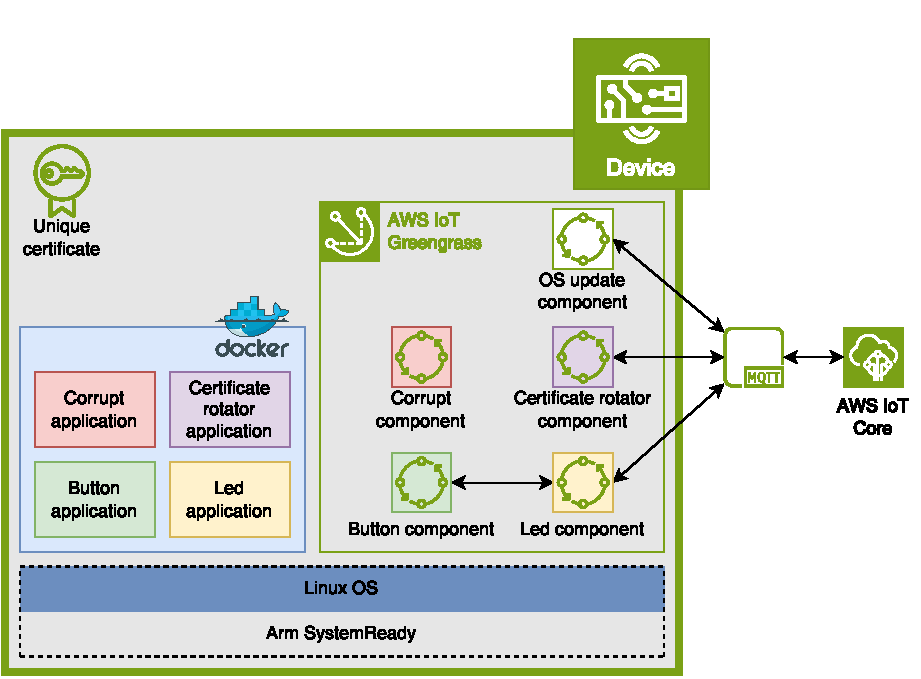
\includegraphics[width=1\columnwidth]{design/apps_overview.pdf}
    \captionof{figure}{Applications overview}
    \label{fig:apps_overview}
    \endgroup
\end{center}

\subsection{\acrshort{os} update}
The application used to update \acrlong{os} features is essential to the reference architecture. Keeping Linux up to date is essential for security, stability, performance and compatibility. Security updates correct vulnerabilities, minimising the risk of exploitation by malicious software. Bug fixes and performance optimisations improve system stability and efficiency. Updating also ensures compliance with security requirements and adaptation to new features and standards. By keeping a Linux \acrshort{os} up to date, users can ensure that their system runs at optimum performance while keeping pace with technological developments and industry requirements.

This application does not run in a Docker container, but directly in the Greengrass component. The operation of the application must be kept simple. An activity diagram in figure \ref{fig:activity_diagram_OS_update} shows this.
\begin{center}
    \begingroup
    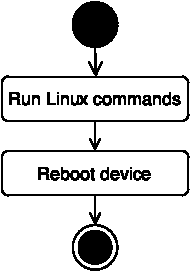
\includegraphics[width=.2\columnwidth]{design/activity_diagram_OS_update.pdf}
    \captionof{figure}{\acrshort{os} update application activity diagram}
    \label{fig:activity_diagram_OS_update}
    \endgroup
\end{center}
When the component starts up the first time the device is launched or after it has been updated, it will execute the Linux commands that have been written. To enable a complete update, the device will restart automatically. The component executes the Linux commands only once for each new version of the component.

\subsection{Certificate rotation}
On embedded systems communicating with \gls{aws}, unique certificates are used to establish secure connections via the protocols. Certificates have expiry dates for security reasons. The use of certificates with an expiry date makes it possible to limit the time during which a certificate is considered valid. This helps to reduce the risks associated with compromised private keys and ensures that certificates are regularly renewed, incorporating the latest security standards. It is therefore crucial to update certificates on embedded systems before their expiry date. If a certificate expires, secure connections with \gls{cloud} services may be interrupted, leading to communication problems. To avoid this, this application must allow certificates to be managed automatically. It works with the \gls{aws} \acrshort{iot} Device Defender service, which alerts the application when it is time to change a certificate.

This application runs in a Docker container. An activity diagram illustrates its behaviour in figure \ref{fig:activity_diagram_certificate_rotator}.
\begin{center}
    \begingroup
    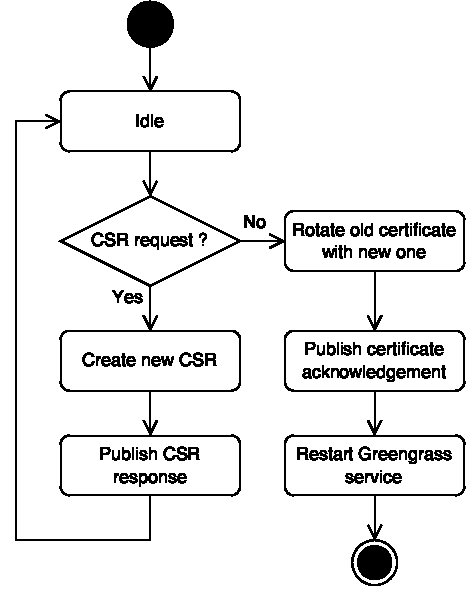
\includegraphics[width=.5\columnwidth]{design/activity_diagram_certificate_rotator.pdf}
    \captionof{figure}{Certificate rotator application activity diagram}
    \label{fig:activity_diagram_certificate_rotator}
    \endgroup
\end{center}
The general idea is that it is alerted by the \gls{aws} \acrshort{iot} Device Defender service when a certificate change is required. The application then creates a new private key and makes a certificate creation request (\acrfull{csr}) to the Amazon root certificate authority. A signed certificate is returned. This will replace the old certificate and the old private key with the new one. In order for the \gls{aws} \acrshort{iot} Greengrass Core service to take the new certificate into account during future communications, this service must be restarted on the device. An overview of the certificate rotation is shown in figure \ref{fig:CertificateRotation_Overview}. It shows the links between the \gls{aws} services and the application on the \acrshort{iot} device.
\begin{center}
    \begingroup
    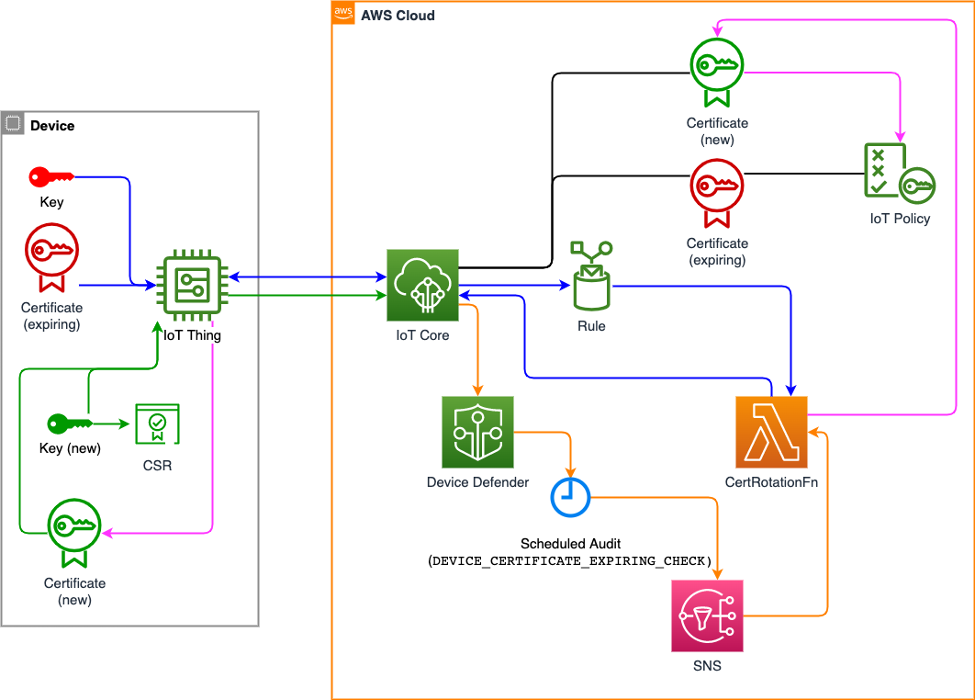
\includegraphics[width=1\columnwidth]{design/CertificateRotation_Overview.png}
    \captionof{figure}{Certificate rotation overview \cite{aws_iot_certificate_rotator}}
    \label{fig:CertificateRotation_Overview}
    \endgroup
\end{center}

\subsection{Led application}
\label{subsec:led_app}
This application is not essential to the reference architecture. It is used as a demonstration for \acrshort{mqtt} communication with \gls{aws} \acrshort{iot}. It is an application in a Docker container that blinks a led on an embedded system. The blinking frequency can be adjusted from an application associated with \gls{aws} \acrshort{iot} using the \acrshort{mqtt} protocol. Blinking can also be enabled or disabled from the \hyperref[subsec:button_app]{button application}. Two pieces of data, the blink frequency and the blink state, are transmitted to \gls{aws} \acrshort{iot} so that they can be viewed on an interface. This is shown in figure \ref{fig:use_case_led_button_apps}.
\begin{center}
    \begingroup
    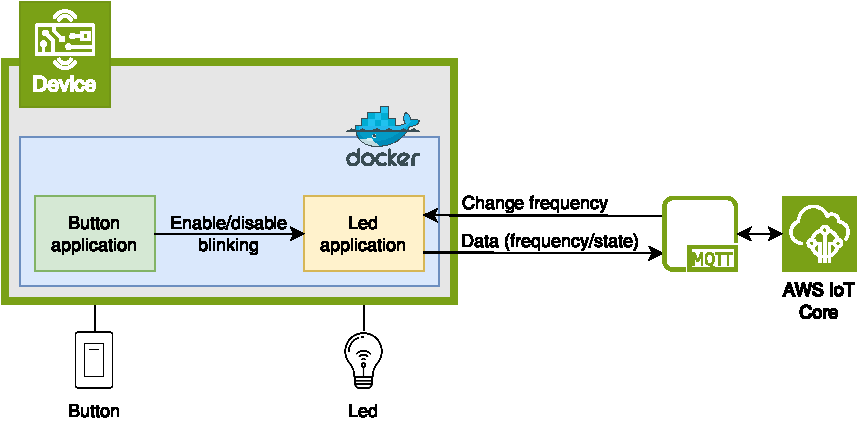
\includegraphics[width=.8\columnwidth]{design/use_case_led_button_apps.pdf}
    \captionof{figure}{Led and button applications interactions}
    \label{fig:use_case_led_button_apps}
    \endgroup
\end{center}

\subsection{Button application}
\label{subsec:button_app}
This application is connected to the \hyperref[subsec:led_app]{led application} while retaining its independence. It is designed as a demonstration of local \acrshort{mqtt} communication. Also running in a Docker container, it simply interacts with the \hyperref[subsec:led_app]{led application} to activate or deactivate the blinking of the led. The user presses a button built into the device to reverse the blinking state. A high-level view is shown in figure \ref{fig:use_case_led_button_apps}.

\subsection{Corrupt application}
A corrupted application is also developed to examine the behaviour of the device with \gls{aws} services. The approach is to run a simple Docker application by deliberately providing an incorrect environment for launching the container.